% Letters
% Letters are short reports of original research focused on an outstanding finding whose importance means that it will be of interest to scientists in other fields.

% They do not normally exceed 4 pages of Nature and, as a guideline, allow up to 30 references. They begin with a fully referenced paragraph, ideally of about 200 words, but certainly no more than 300 words, aimed at readers in other disciplines. This paragraph starts with a 2-3 sentence basic introduction to the field; followed by a one-sentence statement of the main conclusions starting 'Here we show' or equivalent phrase; and finally, 2-3 sentences putting the main findings into general context so it is clear how the results described in the paper have moved the field forwards.

% Please refer to our annotated example to see how the summary paragraph for a Letter should be constructed.

% The rest of the text is typically about 1,500 words long. Any discussion at the end of the text should be as succinct as possible, not repeating previous summary/introduction material, to briefly convey the general relevance of the work.

% Letters typically have 3 or 4 small display items (figures or tables).

% Word counts refer to the text of the paper. References, title, author list and acknowledgements do not have to be included in total word counts.

%%%%%%%%%%%%
% GAMEPLAN %
%%%%%%%%%%%%

%%%%%%%%%%%%%%%
%% MAIN TEXT %%
%%%%%%%%%%%%%%%

% introduction to the question of IA
% topography, climate, and lithology are important
% GEOCLIM model
% dependence on slope and lithology
% calibration (various feasible combinations of parameters)
% temperature and runoff from GFDL
% tested scenarios, including explanation of the paleoshoreline data
% IA is important, traps are less important
% limitations with approach
    % GFDL equilibrated by last 100 years?
    % not changing paleogeography
    % source term. Can cite: Rowan2016a related to spreading rate.
    % low resolution
    % GFDL model is quite old
    % kinetics are not changing between lithologies
    
%%%%%%%%%%%%%%%%%%%%%%%
%% MAIN TEXT FIGURES %%
%%%%%%%%%%%%%%%%%%%%%%%

% paleoshorelines
% steady state pCO2 for all scenarios

%%%%%%%%%%%%%%%%%%%%%%%%%%%%%%%
%% SUPPLEMENTARY INFORMATION %%
%%%%%%%%%%%%%%%%%%%%%%%%%%%%%%%

% details of DynSoil and GEOCLIM
% details of parameter exploration/calibration
    % basin data used for parameter exploration
% details of lithology implementation
    % including Sunda Shelf
% details of paleoshoreline reconstructions

%%%%%%%%%%%%%%%%%%%%%%%%%%%%%%%%%%%%%%
%% SUPPLMENTARY INFORMATION FIGURES %%
%%%%%%%%%%%%%%%%%%%%%%%%%%%%%%%%%%%%%%

% regolith model schematic
% maps of all scenarios

\documentclass[11pt,letterpaper]{article}

%\usepackage{fontspec}
%\usepackage[utf8]{inputenc}
\usepackage{textcomp,marvosym}
\usepackage{amsmath,amssymb}
\usepackage[normalem]{ulem}
\usepackage[left]{lineno}
\usepackage{booktabs}
\usepackage{changepage}
\usepackage{rotating}
\usepackage{color}
\usepackage{natbib}
\usepackage{setspace}
\usepackage{array}
\usepackage{fancyhdr}
\usepackage{graphicx}
\usepackage{xspace}
\usepackage[hidelinks]{hyperref}
\urlstyle{same}
\usepackage{threeparttable}
\doublespacing

\raggedright
\textwidth = 6.5 in
\textheight = 8.25 in
\oddsidemargin = 0.0 in
\evensidemargin = 0.0 in
\topmargin = 0.0 in
\headheight = 0.0 in
\headsep = 0.5 in
\parskip = 0.1 in
\parindent = 0.2in

% Bold the 'Figure #' in the caption and separate it from the title/caption with a period
% Captions will be left justified
\usepackage[aboveskip=1pt,labelfont=bf,labelsep=period,justification=raggedright,singlelinecheck=off]{caption}

% Remove brackets from numbering in List of References
%\makeatletter
%\renewcommand{\@biblabel}[1]{\quad#1.}
%\makeatother

% Self defined commands
\newcommand{\degreesC}{\textdegree C\xspace}
\newcommand{\degrees}{\textdegree\xspace}
\newcommand{\dC}{$\delta^{13}$C\xspace}
\newcommand{\dO}{$\delta^{18}$O\xspace}
\newcommand{\SrSr}{$^{87}$Sr/$^{86}$Sr\xspace}
\newcommand{\permil}{\textperthousand\xspace}
\newcommand{\UPb}{$^{206}$Pb/$^{238}$U\xspace}
\newcommand{\pCOtwo}{\textit{p}CO$_{2}$\xspace}
\newcommand{\COtwo}{CO$_{2}$\xspace}
%

\pagestyle{myheadings}
\pagestyle{fancy}
\fancyhf{}
\lhead{Park et al., in preparation}
\rhead{\thepage}

\begin{document}

\begin{flushleft}
{\Large \textbf{Emergence of Indonesia and New Guinea as a driver for Neogene cooling}}

Yuem Park\textsuperscript{1},
Nicholas L. Swanson-Hysell\textsuperscript{1},
Pierre Maffre\textsuperscript{1},
Francis A. Macdonald\textsuperscript{2},
Eliel A. Anttila\textsuperscript{2},
Yves Godd\'eris\textsuperscript{3}

\bigskip
\textsuperscript{1} Department of Earth and Planetary Science, University of California, Berkeley, CA, USA

\textsuperscript{2} Department of Earth Science, University of California, Santa Barbara, CA, USA

\textsuperscript{3} G\'eosciences Environnement Toulouse, CNRS--Universit\'e Paul Sabatier - IRD, Toulouse, France

\bigskip

\end{flushleft}

\linenumbers

Indonesia and New Guinea (I\&NG) have an outsized influence on modern chemical weathering fluxes. The confluence of steep topography, a warm and wet tropical climate, and the presence of mafic lithologies results in high fluxes of Ca and Mg cations and associated \COtwo consumption \citep{Gaillardet1999a, Hartmann2009a, Hartmann2014a}. There has been a significant increase of subaerially-exposed land area within the region since the Miocene associated with ongoing arc-continent collision between Australia and the Sunda-Banda Arc system (\citealp{Molnar2015a, Hall2017a}; Fig. \ref{fig:shoreline_growth}). The collision between the Australian-Indian and Eurasian plates and intervening arc terranes has led to the emergence of I\&NG and the exhumation of large supra-subduction ophiolites and associated forearcs in the warm, wet tropics \citep{Macdonald2019a}.

Given that the region is a modern-day hot spot of fresh water and sediment discharge \citep{Milliman2013a} and chemical weathering and \COtwo consumption \citep{Hartmann2009a}, what effect has the emergence of I\&NG had on Earth's geochemical cycles and climate state? If this region was instead under water, would we have a glacial climate today? Based on paleogeographic reconstructions of arc-continent collisions through time, \citet{Macdonald2019a} proposed that arc-continent collisions in the tropics are responsible for increasing planetary weatherability, lowering \pCOtwo and causing the onset of glacial climate states. After the Miocene Climatic Optimum (MCO), a cooling trend began at $\sim$14~Ma associated with the growth of the Antarctic ice sheet, and accelerated over the past 4~m.y. culminating with the onset of northern hemisphere glaciation \citep{Shackleton1984a, Zachos2001a}. The \pCOtwo threshold for Antarctic glaciation is estimated to be $\sim$750~ppm with that for northern hemisphere glaciation being significantly lower at $\sim$280~ppm \citep{DeConto2008a}. The lower \pCOtwo threshold for northern hemisphere glaciation provides an explanation for southern hemisphere glaciation significantly preceding the development of ice sheets in both hemispheres. We seek to evaluate the hypothesis that the increase of subaerially-exposed land area in I\&NG has played a significant role in lowering \pCOtwo thereby driving this cooling and the development of northern hemisphere ice sheets.

Over geologic time-scales, \COtwo enters Earth's ocean/atmosphere system primarily via volcanism and metamorphic degassing of the solid Earth, and leaves it primarily through the chemical weathering of silicate rocks, which delivers alkalinity and cations to the ocean that ultimately result in the consumption of carbon via the precipitation of carbonate rocks \citep{Kump2000a}. However, assessing the effect of the emergence of I\&NG on Earth's \pCOtwo levels can not be determined simply through assessing the present-day chemical weathering fluxes. The steady-state \pCOtwo of Earth is set by the \pCOtwo level at which the sinks of \COtwo are equal to the sources. For example, as \COtwo sinks are removed and \COtwo rises, temperature increases and the hydrological cycle is invigorated, which causes other weathering sinks to increase until a new steady-state is achieved at a higher \pCOtwo. Conversely, the magnitude of the silicate weathering \COtwo sink can be equal to the magnitude of the source at lower steady-state \pCOtwo on a planet with relatively high weatherability than on a planet where it is lower \citep{Kump1997a}.

Topography, climate, and lithology all play important roles in modulating chemical weathering. In low-relief regions, low physical erosion rates lead to a supply-limited weathering regime, in contrast to regions of high denudation where there are higher weathering fluxes \citep{Gabet2009a, West2012a, Maher2014a}. In warm and wet regions, mineral dissolution kinetics are faster leading to enhanced chemical weathering \citep{Lasaga1994a, West2012a}. Regions with high physical weathering rates that are not supply-limited are more sensitive to changes in climate that can enhance the total chemical weathering rate \citep{West2012a, Maher2014a}. In terms of lithology, mafic rocks have the potential to sequester more carbon through silicate weathering because of their relatively high concentrations of Ca and Mg as well as high reaction rates \citep{Dessert2003a}. These factors are what have lead to the proposal that arc-continent collisions within the tropical rain belt have been important in enhancing global weatherability, lowering atmospheric \pCOtwo and initiating glacial climate over the past 520~m.y. \citep{Jagoutz2016a, Swanson-Hysell2017a, Macdonald2019a} and perhaps in the Neoproterozoic as well \citep{Park2019a}.

To estimate the decrease in steady state \pCOtwo associated with the increase in global weatherability associated with the increase of subaerially-exposed land area in I\&NG, we use the spatially-resolved GEOCLIM model \citep{Godderis2014a, Godderis2017c} wherein a silicate weathering model is coupled to global climate models run at varying \pCOtwo levels. We use the DynSoil implementation of the \citet{Gabet2009a} regolith development model which integrates a climatic dependence on chemical weathering using the formulation of \cite{West2012a}.

The silicate weathering component of GEOCLIM calculates \COtwo consumption by silicate weathering for each continental grid cell. In previous versions of the model, the silicate weathering rate was a function of temperature and runoff only, and assumed that the bedrock in all continental grid cells had identical chemical compositions (e.g. \citealp{Godderis2014a}). However, more recent versions of GEOCLIM implement regolith development and soil shielding into the silicate weathering component based on work by \citet{Heimsath1997a}, \citet{Gabet2009a}, \citet{West2012a}, \citet{Carretier2014a}, \citet{Godderis2017b}, and \citet{Maffre2018a}, which introduces an additional dependence on topographic slope (see SI). While this introduction of regolith development into GEOCLIM is an important piece of assessing the impact of tropical arc-continent collisions on \pCOtwo, the relatively high Ca+Mg concentration in arc rocks relative to other lithologies must also be considered. We therefore implement variable bedrock Ca+Mg concentration into the silicate weathering component of GEOCLIM. The spatial distribution of lithologies is sourced from the global lithologic map (GLiM) of \citet{Hartmann2012a} with the 16 lithologic categories represented in GLiM grouped into 6 broader categories: metamorphic, felsic, intermediate, mafic, carbonate, and siliciclastic sediment (Fig. SX). Each continental grid cell is assigned one of these lithologic categories at a resolution of 0.1\degrees $\times$ 0.1\degrees. The Ca+Mg concentrations of felsic, intermediate, and mafic grid cells are then assigned based on the mean of MgO and CaO measurements on rocks of each of these lithologic categories in data compiled from the EarthChem Portal (\url{www.earthchem.org/portal}). The weathering of carbonate grid cells does not contribute to long-term \COtwo consumption and therefore its Ca+Mg concentration is ignored in this analysis. The Ca+Mg concentrations of metamorphic and siliciclastic sediment grid cells are more difficult to define, since the chemical composition of these two lithologic classes is strongly dependent on its protolith. The chemical composition of siliciclastic sediment is further strongly dependent on its degree of chemical depletion. We therefore explore a range of feasible Ca+Mg concentrations of metamorphic and siliciclastic sediment grid cells during the calibration of the silicate weathering component of GEOCLIM (see below).

Of the various parameters used in the equations that govern the silicate weathering component of GEOCLIM (see SI), four parameters in particular are poorly constrained in the existing literature: the proportionality constant that modifies the dependence of dissolution rate on runoff and temperature ($k_{d}$), the proportionality constant that modifies the dependence of dissolution rate on runoff only ($k_{w}$), the power constant that modifies the dependence of dissolution rate on the time that a rock particle has spent in the regolith ($\sigma$), and the proportionality constant that modifies the dependence of regolith production on runoff and temperature ($k_{rp}$). As discussed above, the Ca+Mg concentrations of metamorphic and siliciclastic sediment grid cells are also difficult to define. Rather than prescribing values for these six parameters, we instead allow these parameters to vary within reasonable bounds, resulting in a total of 78,000 unique parameter combinations. For each of these combinations, we compute spatially-resolved long-term \COtwo consumption (i.e. Ca+Mg consumption) using present-day runoff, temperature, and slope fields. Following the approach of \citet{Maffre2018a}, we then sum the computed \COtwo consumption over large-scale watersheds that appear in the global compilation of \citet{Gaillardet1999a}, as well as smaller-scale watersheds of the Amazon Basin in the compilation of \citet{Moquet2011a, Moquet2016a, Moquet2018a}. We then calculate the coefficient of determination ($r^{2}$) between computed and measured \COtwo consumption in each of these basins. We eliminate all parameter combinations that result in unreasonable total global \COtwo consumption (which we define to be \textless1$\times$10$^{12}$~mol/yr or \textgreater1$\times$10$^{13}$~mol/yr) and/or result in a low $r^{2}$ (which we define to be \textless0.4). This calibration method leaves 3,339 unique parameter combinations that produce global and individual watershed \COtwo consumption fluxes that approximate those estimated in the literature for the present-day.

Having calibrated the silicate weathering component of GEOCLIM, we estimate the decrease in steady-state \pCOtwo associated with increases in global weatherability. To do so, we use temperature and runoff fields from a subset of the GFDL CM2.0 experiments \citep{Delworth2006a, Delworth2006b} for the climate model component of GEOCLIM. These experiments were performed in order to explore the effect of various changes in forcing agents on climate since ca. 1860 at a 1\degrees $\times$ 1\degrees resolution. In the ``1860 control'' experiment, forcing agents representative of conditions ca. 1860 (including \COtwo, CH$_{4}$, N$_{2}$O, O$_{3}$, sulfates, carbon, dust, sea salt, solar irradiance, and the distribution of land cover types) are held constant for 500 years after reaching equilibrium. \pCOtwo in 1860 is assumed to be 286~ppm. In the ``+1\%/yr to 2$\times$'' experiment, initial conditions are taken from the ``1860 control'' experiment, then \pCOtwo is prescribed to increase from 286~ppm at a compounded rate of +1\% per year for 70 years, when \pCOtwo reaches double (572~ppm) of the initial value. \pCOtwo is then held constant until the end of the 280 year experiment. All non-\COtwo forcing agents are held constant. The ``+1\%/yr to 4$\times$'' experiment is identical to the ``+1\%/yr to 2$\times$'' experiment, except that \pCOtwo is prescribed to increase for 140 years, when \pCOtwo reaches quadruple (1144~ppm) of the initial value. We take the mean of the last 100 years of each of these three experiments (when \pCOtwo is being held constant at its final level) to obtain temperature and runoff fields for 286, 572, and 1144~ppm respectively. The primary strength of using these three GFDL CM2.0 experiments is that all non-\COtwo forcing agents are held constant, allowing the effect of \pCOtwo on climate to be isolated.

We use geological and paleoshoreline data to quantify the changes in the area of I\&NG over the past 20~m.y. (Fig. \ref{fig:shoreline_growth}). Following \citet{Molnar2015a}, we analyzed the area changes of islands that are greater than $\sim$200~km$^{2}$, and we also included changes in areas of submerged continental shelves that were previously exposed, like the Sunda Shelf. Carbonate strata and thin-bedded siliciclastic strata were interpreted to represent a subaqueous marine environment, whereas evidence for exposure and terrestrial siliciclastic deposits were used as evidence for a subaerial environment. Taken together, these constraints delineate the position of shorelines. For the island of Sulawesi, we followed the recent stratigraphic compilation and paleoshorelines delineated by \citet{Nugraha2018a} and for New Guinea we followed work of \citet{Norwick2003a, Harrington2017a, Gold2017a}. Although there are difference in data sources and paleoshoreline outlines from \cite{Molnar2015a}, the calculated area at 5~Ma is similar.

Along with the Neogene increase in subaerially-exposed land area and tectonic topography associated with arc-continent collision, there has also been a decrease in subaerially-exposed land area on the Sunda Shelf \citep{Sarr2019a}. Large portions of this low-relief area of continental crust were likely emergent throughout the Neogene, and were repeatedly subaerially exposed during the Pleistocene as recently as the Last Glacial Maximum \citep{Hall2002a}, potentially driving climate amplification on orbital timescales \citep{DiNezio2018a}. Similarities in terrestrial biotas of Borneo and mainland Southeast Asia suggest the existence of land bridges on the Sunda Shelf throughout the Miocene \citep{Moss1998a}. During the Eocene through early Miocene, the rifting of the South China Sea resulted in subsidence of the Sunda Shelf \citep{Morley2013a} and recent subsidence is interpreted to be a result of dynamic topography, triggered by subduction-related mantle flow \citep{Sarr2019a}. In the Miocene, this region exposed a mixture of felsic basement rocks and siliciclastic sediments \citet{Darmadi2007a}. The relatively low-relief and felsic lithologies of the region contrasts with the high-relief and mafic lithologies of most of I\&NG.

To explore the sensitivity of global weatherability and climate state to the emergence of I\&NG, we test three scenarios using GEOCLIM (Fig. \ref{fig:scenario_pCO2}). The ``removed I\&NG'' scenario represents an end-member scenario, in which all islands associated with arc-continent collision in the area are entirely removed. The ``reduced I\&NG'' scenario represents our best estimate of the subaerial extent of islands in the area at ca. 15~Ma, excluding the Sunda Shelf. The ``reduced I\&NG + Sunda Shelf'' is identical to the ``reduced I\&NG'' scenario with the addition of the Sunda Shelf. Given that no land in the Sunda Shelf is currently exposed, across the shelf we distribute felsic and siliciclastic lithologies, assign shallow slope values, and interpolate runoff across latitude bands (see SI).

Using the 3,339 unique parameter combinations, the ``removed I\&NG'' scenario resulted in steady-state \pCOtwo's of 598-729~ppm (5-95 percentile values), the ``reduced I\&NG'' scenario of 547-638~ppm, and the ``reduced I\&NG + Sunda Shelf'' of 533-611~ppm (Fig. \ref{fig:scenario_pCO2}). These results suggest that without the Neogene increase in subaerially-exposed land area and tectonic topography associated with arc-continent collision, pre-Industrial \pCOtwo would have been $\sim$500-700~ppm. Notably, the effect of the Sunda Shelf on steady-state \pCOtwo is relatively small, given the low Mg+Ca concentration of the lithologies that comprise the Sunda Shelf as well as its low slope. These GEOCLIM \pCOtwo values resemble the higher end of proxy-based \pCOtwo estimates for the early Miocene \citep{Foster2017a}, indicating that the increase in subaerially-exposed land area and tectonic topography of I\&NG is itself sufficient to explain climate change over the Neogene.

I\&NG are potent sinks of carbon because they contain large swaths of ophiolites that are exposed along E-W belts of tectonic topography in the warm wet tropics. In New Guinea, these paleogeographic features originated in the Middle Miocene with the collision between the Melanesian Arc and the distal margin of Australia \citep{vanUfford2005a, Cloos2005a, Baldwin2012a}, which resulted in the exhumation of the 1440~km long Irian-Marum-April Ophiolite Belt. The Middle Miocene (16-14~Ma) basal Markats Formation contains siliciclastic sediment that was transported from the south into the forearc basin associated with the New Guinea ophiolite belt \citep{Cloos2005a}. This precedes, by several million years, the beginning of widespread synorogenic sedimentation to the south and on the Australian continental basement at ca. 12~Ma \citep{vanUfford2005a}. Exhumation of the Central Range accelerated over the past 4~m.y. due to slab-breakoff and buoyant uplift under New Guinea \citep{Cloos2005a}. After arc-continent collision in New Guinea, a left-lateral strike-slip margin developed on the northern margin \citep{Baldwin2012a}. Over the past 4~m.y., this change in plate motion caused the westward extrusion and exhumation of the Cretaceous to Oligocene ophiolites of Obi, Halmahera, and northern New Guinea \citep{Baldwin2012a}. In eastern New Guinea, progressive jamming of the north-dipping subduction zone has caused major uplift over the past 4~m.y. \citep{vanUfford2005a}, which is well dated with a change in provenance from continental to volcanic detritus (Abbott et al., 1994) and thermochronology (Hill \& Gleadow, 1989). 

Most of the non-volcanic islands of the Outer Banda Arc emerged after 5~Ma, associated with slab roll-back and collision with the Australian continental margin \citep{Harris2006a, Hall2013a}. In Timor and Sumba arc-continent collision resulted in rapid uplift of deep marine sedimentary rocks to elevations \textgreater1~km above sea level with estimated average uplift rates of 1.5~km/m.y. (Audley-Charles, 1986).

Our paleoshoreline reconstructions show a broad increase in exposed land area over the Neogene and an acceleration over the past 4~m.y. This trend is due to progressive arc-continent collision from west to east that has culminated with increased exhumation in the Banda Arc and New Guinea in the past 4~m.y. This trend mirrors broad cooling over the Neogene and accelerated cooling over the past 4~m.y that culminated in the initiation of the Northern Hemisphere ice sheets. Not only does the timing of the increase in subaerially-exposed land area of I\&NG coincide with the cooling trend, but our coupled weathering-climate model demonstrates that the magnitude of change in \pCOtwo due to these changes is sufficient to explain climate change over the Neogene.

The movement of the Deccan Traps into the tropical rain belt together with the low-latitude emplacement of the Ethiopian Traps is an hypothesis that has been put forth to explain the draw-down of \COtwo leading into Oligocene glaciation of Antarctica \citep{Kent2008a, Kent2013a}. To explore the sensitivity of global weatherability and climate state to the presence of the surface exposure of basaltic lavas, we test three additional scenarios using GEOCLIM (Fig. \ref{fig:scenario_pCO2}). In the ``removed Deccan Traps'' and the ``removed Ethiopian Traps'' scenarios, all volcanics associated with the respective igneous provinces are replaced with the Ca+Mg concentration of bulk continental crust. In the ``removed both traps'' scenario, all volcanics associated with both provinces are replaced with the Ca+Mg concentration of bulk continental crust. These scenarios result in steady-state \pCOtwo's \textless500~ppm, distinctly lower than those for the three I\&NG scenarios. This result indicates that, while the presence of high Ca+Mg concentration mafic rocks in low-latitude igneous provinces provides a non-negligible contribution to modulating steady-state \pCOtwo, its contribution is significantly smaller than that of high-relief I\&NG.

However, it is important to acknowledge the limitations of the approach taken in this study. First, the tested scenarios only simulate changes in the location of the shorelines in I\&NG and the lithology exposed in the Deccan and Ethiopian Traps. Changes in paleogeography that are not accounted for in our simulations may have resulted in changes in oceanic and atmospheric circulation \citep{Haug1998a, Shevenell2004a, Holbourn2015a, Molnar2015a} that contributed to changes in \pCOtwo on hundreds of thousands to million-year timescales. However, the global extent and multi-million year timescale of the long-term cooling trend since 14~Ma suggests that the primary driver for this cooling is changes in the geological sources and sinks of carbon, modulated by the silicate weathering feedback \citep{Walker1981a, Raymo1991a, Berner1997a, Kump1997a, Berner2001a}. In this way, changes in the flux of \COtwo outgassing via changes in spreading rates and ridge lengths \citep{Rowan2016a} and changes in weatherability via mountain building and the movement of land masses into/out of areas of high temperature and runoff are likely more important paleogeography-related factors in terms of modulating Neogene cooling than changes in oceanic and atmospheric circulation. Second, the climate model component of GEOCLIM that was used in this study (GFDL CM2.0) has a low spatial resolution (2.0\degrees $\times$ 2.5\degrees) and is based upon physics and geochemical cycles that have been superceded by more recent climate models. Using an updated climate model at higher resolution may result in runoff and temperature fields with different sensitivities to paleogeography and \pCOtwo. Finally, although the silicate weathering component of GEOCLIM now implements lithology-dependent Ca+Mg concentration, it does not yet implement lithology-dependent kinetics of mineral dissolution. Nevertheless, relative to felsic lithologies, mafic lithologies more dominantly comprise of minerals with faster kinetics (e.g. olivine and plagioclase; see SI), and thus incorporating lithology-dependent kinetics of mineral dissolution into our simulations would likely increase the sensitivity of steady-state \pCOtwo to increases in subaerially-exposed land area and tectonic topography of I\&NG.


%%% RELATIVELY COMPLETE TEXT ABOVE - BELOW ARE SNIPPETS THAT COULD BE INCORPORATED IN

%%%

%After the MCO, a cooling trend began ca. 14~Ma that accelerated over the past 4~m.y. Many hypotheses have been proposed to explain this cooling trend including changes in ocean circulation and upwelling \citep{Shevenell2004a, Holbourn2015a}, perhaps associated with increased organic carbon burial \citep{Vincent1985a, Flower1993a} or the closure of the Central American Seaway \citep{Haug1998a}, an increase in the strength of the Walker Circulation \citep{Molnar2015a}, feedbacks with terrestrial vegetation \citep{Cerling1997a}(MAYBE ONE OF THE DINEZIO REFS), uplift in the Himalayas \citep{Raymo1988a}, or a decrease in volcanic outgassing \citep{Berner1983a}(ROWAN+ROWLEY). Although changes in circulation and vegetation may have contributed to changes in \pCOtwo on hundreds of thousands to million-year timescales, the global extent and multi-million year timescale suggests that the long-term cooling trend since 14~Ma is the product of changes in the geological sources and sinks of carbon, modulated by the silicate weathering feedback \citep{Walker1981a, Raymo1991a, Berner1997a, Kump1997a, Berner2001a}. Global spreading rates, ridge length, and paleogeography elsewhere on Earth undoubtedly changed through the Neogene contributing to changes in geological carbon sources and sinks, however, here we show that the global climate state is particularly sensitive to the tropical paleogeograpahy of I\&NG.

\section*{ACKNOWLEDGEMENTS \label{sec:ACKNOWLEDGEMENTS}}

We thank Alec Brenner, Sam Lo Bianco, Mariana Lin, and Judy Pu for their contributions to the paleoshoreline reconstructions. Collaborative research between NLS-H and YG was initially supported by the France-Berkeley Fund. FAM and NLS-H thank NSF FRES grant \#20191023 for support. 

\clearpage
\newpage

\section*{FIGURES}

\begin{figure}[h!]
    \centering
    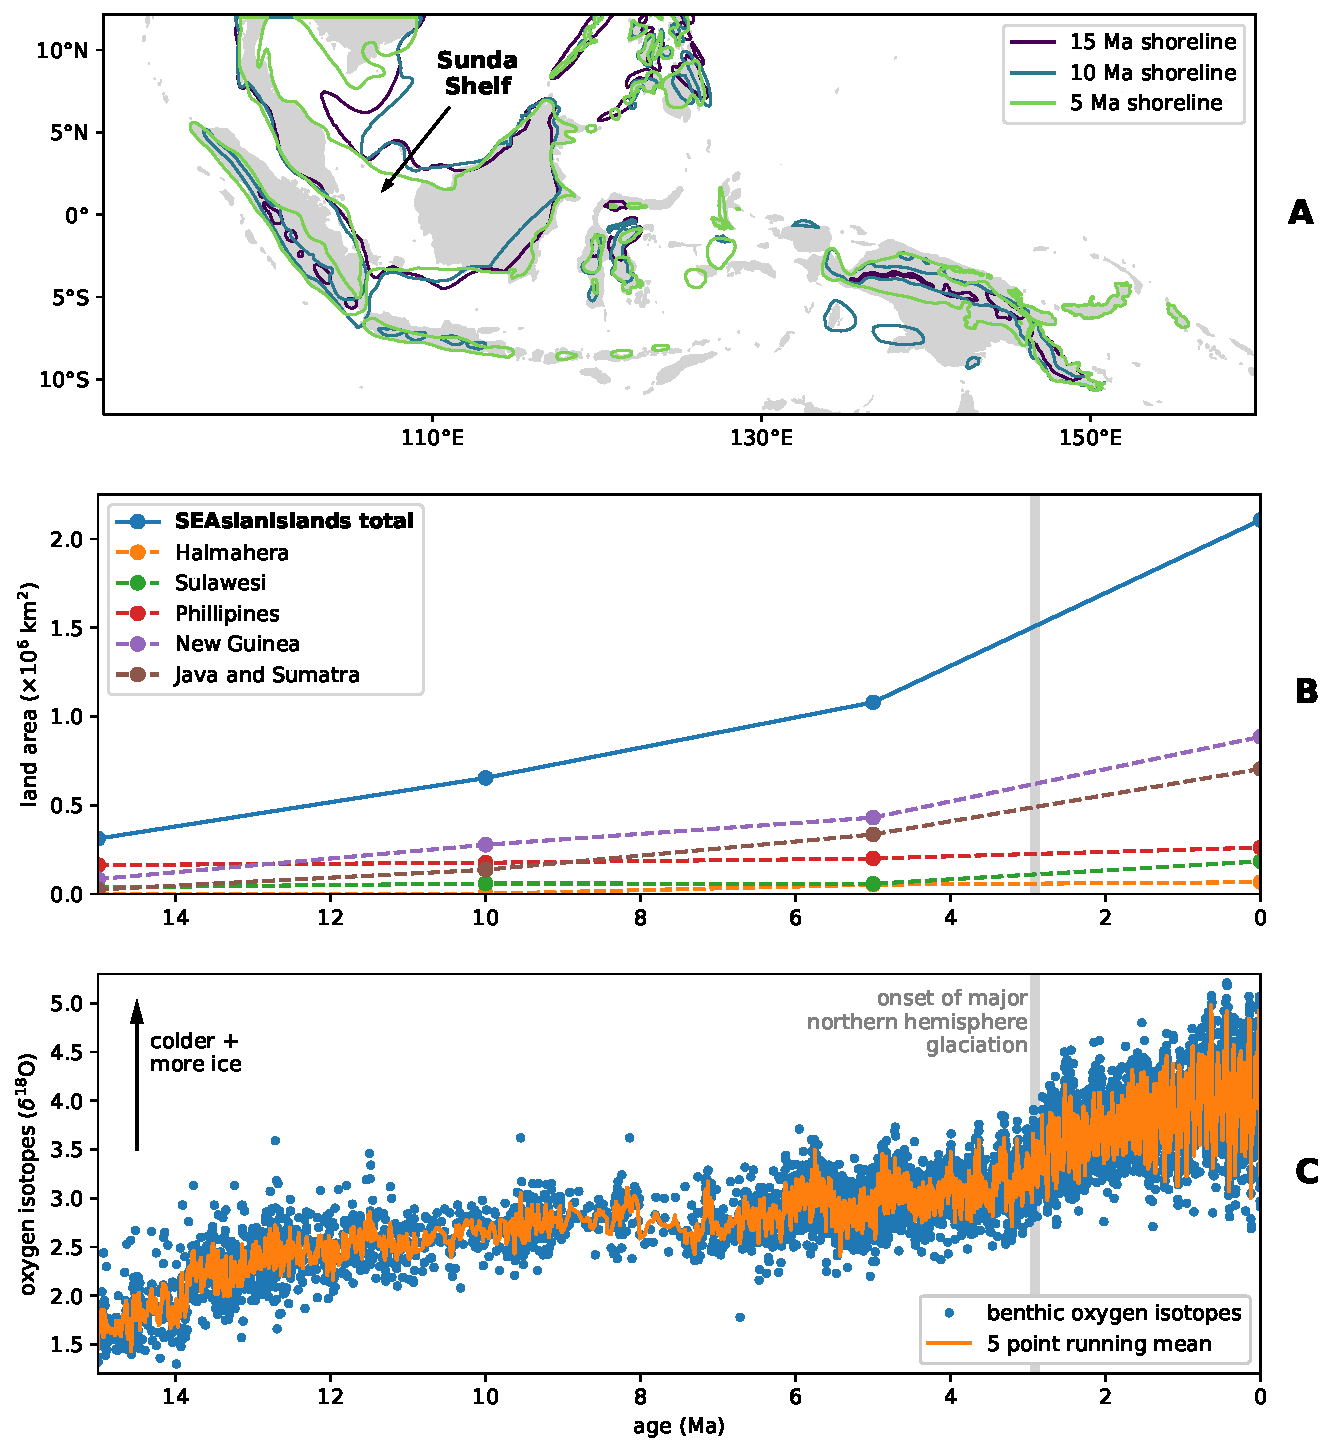
\includegraphics[width=0.9\textwidth]{Manuscript/Figures/shoreline_growth.pdf}
    \caption{The emergence of Indonesia and New Guinea. Past shorelines are shown in A with resultant area estimates summarized in B. A significant increase in area over the past 4 million years is coincident with cooling and the onset of Northern Hemisphere glaciation as reflected in the benthic oxygen isotope record in C \citep{Zachos2008a}.}
    \label{fig:shoreline_growth}
\end{figure}

\begin{figure}[h!]
    \centering
    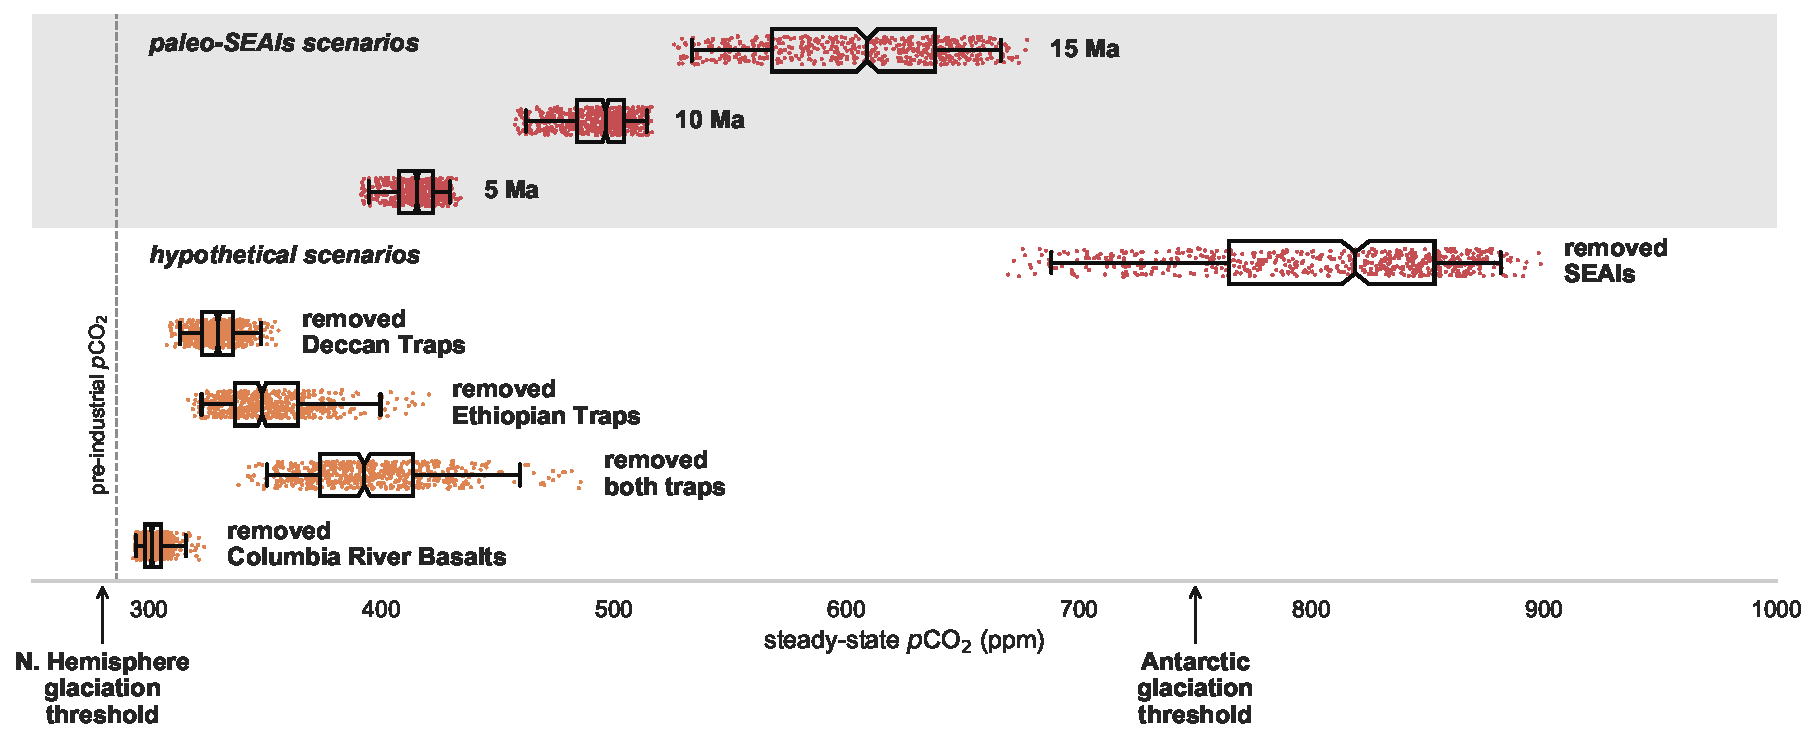
\includegraphics[width=1\textwidth]{Manuscript/Figures/scenario_pCO2.pdf}
    \caption{Box shows quartiles, whiskers show 1.5$\times$ the interquartile range, notch shows median with 95\% confidence interval. Each dot shows a parameter combination. Dashed line is PI \pCOtwo.}
    \label{fig:scenario_pCO2}
\end{figure}

\clearpage
\newpage
\footnotesize

\singlespacing

\bibliographystyle{gsabull}
\bibliography{References}

\end{document}